% The teaser is placed under the title block on the first page. A figure* cannot
% appear on the page where it is defined in two-column mode, so the figure is
% appended to the title block that spconf typesets with \twocolumn[...].
\makeatletter
\g@addto@macro\@maketitle{%
  \begin{center}
  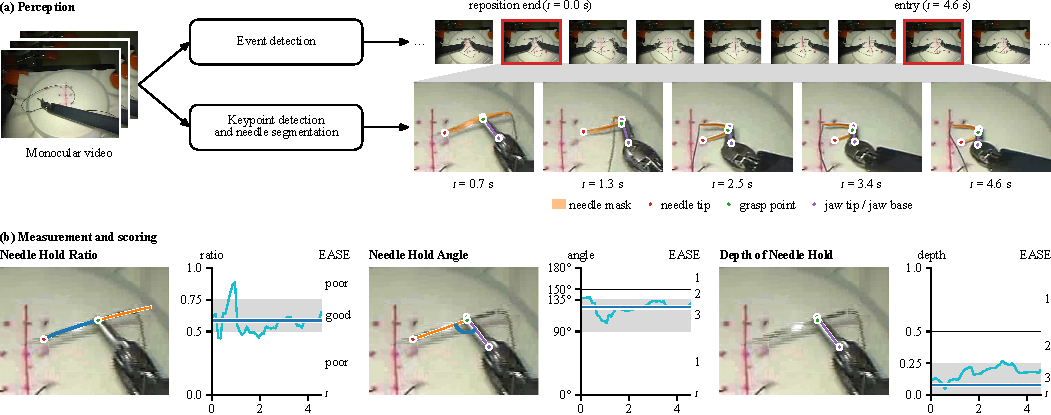
\includegraphics{figures/overview}%
  \refstepcounter{figure}%
  \def\@captype{figure}%
  \@makecaption{\fnum@figure}{Overview of the method. (a) Perception. Events are detected
    in the monocular suturing video; they divide it into stitches and into the window
    that each sub-skill refers to. Top: frames of one stitch; the reposition end and the
    entry (red frames) delimit the hold window (gray). Bottom: enlarged frames of the
    window with the detected keypoints and needle mask; $t$ is the time from the
    reposition end in seconds. (b) Measurement and scoring, for the same stitch. For
    each sub-skill, the measured geometry is drawn on a frame of the window (blue: what
    is measured; orange: the needle; purple: the jaws), and the estimate of every frame
    of the window is plotted over time against the EASE score ranges. Cyan: the
    estimate of each frame; blue with a white edge: the value used, namely the ratio
    fitted to all frames of the window at once (cyan: fitted to each frame alone), the
    median of the angles, and the depth in the frame in which the jaws appear longest,
    which is the frame shown. Gray: the range of the EASE ground truth of this stitch;
    the labels at the right are the scores of the ranges.}%
  \label{fig:overview}
  \end{center}
  \vskip 1em}
\makeatother
